\documentclass[12pt,a4paper,onecolumn]{article}
\usepackage[utf8]{inputenc}
\usepackage[T1]{fontenc}
\usepackage[french]{babel}

% ------------------------- Color table ----------------------------------------
\usepackage{multirow}
\usepackage[table]{xcolor}
\definecolor{maroon}{cmyk}{0,0.87,0.68,0.32}
% ------------------------------------------------------------------------------

\usepackage{amscd}
\usepackage{amsthm}
\usepackage{physics}
\usepackage[left=2.2cm,right=2.2cm,top=2cm,bottom=2cm]{geometry}
\usepackage{textcomp,gensymb} %pour le °C, et textcomp pour éviter les warning
\usepackage{graphicx} %pour les images
\usepackage{caption}
\usepackage{subcaption}
\usepackage[colorlinks=true,
	breaklinks=true,
	citecolor=blue,
	linkcolor=blue,
	urlcolor=blue]{hyperref} % pour insérer des liens
\usepackage{epstopdf} %converting to PDF
\usepackage[export]{adjustbox} %for large figures

\usepackage{array}
\usepackage{dsfont}% indicatrice : \mathds{1}


% -------------------------- Mathematics ---------------------------------------
\graphicspath{{images/}{../images/}} % For the images path
% ------------------------------------------------------------------------------

% -------------------------- Mathematics ---------------------------------------
\usepackage{mathrsfs, amsmath, amsfonts, amssymb}
\usepackage{bm}
\usepackage{mathtools}
\usepackage[Symbol]{upgreek} % For pi \uppi different from /pi
\newcommand{\R}{\mathbb{R}} % For Real space

% ------------------------------------------------------------------------------


% -------------------------- Code format ---------------------------------------
\usepackage[numbered,framed]{matlab-prettifier}
\lstset{
	style              = Matlab-editor,
	basicstyle         = \mlttfamily,
	escapechar         = '',
	mlshowsectionrules = true,
}
% ------------------------------------------------------------------------------

% ------------------------- Blbiographie --------------------------------------
\usepackage[backend=biber, style=ieee]{biblatex}
\addbibresource{biblio.bib}
% ------------------------------------------------------------------------------


\setcounter{tocdepth}{4} %Count paragraph
\setcounter{secnumdepth}{4} %Count paragraph
\usepackage{float}

\usepackage{graphicx} % for graphicspath
% \graphicspath{{../images/}}

\usepackage{array,tabularx}
\newcolumntype{L}[1]{>{\raggedright\let\newline\\\arraybackslash\hspace{0pt}}m{#1}}
\newcolumntype{C}[1]{>{\centering\let\newline\\\arraybackslash\hspace{0pt}}m{#1}}
\newcolumntype{R}[1]{>{\raggedleft\let\newline\\\arraybackslash\hspace{0pt}}m{#1}}

% to start counting section to 6


% ------------------------ General informations --------------------------------
\title{MVA - Recvis - Oral}
\author{Vincent Matthys}
\graphicspath{{images/}{../images/}} % For the images path
% ------------------------------------------------------------------------------


\begin{document}

\begin{tabularx}{0.9\textwidth}{@{} l X r @{} }
	{\textsc{Master MVA}}  &  & \textsc{Vincent Matthys} \\
	\textsc{Recvis} &  & {ENS Paris Saclay}       \\
\end{tabularx}
\vspace{1.5cm}
\begin{center}

	\rule[11pt]{5cm}{0.5pt}

	\textbf{\LARGE \textsc{Tools for oral presentation}}
	\vspace{0.5cm}

	Vincent Matthys

	vincent.matthys@ens-paris-saclay.fr

	\rule{5cm}{0.5pt}

	\vspace{1.5cm}
\end{center}

\section{Bibliography}
\begin{itemize}
	\item Linear model to map 3D joints onto 2D joints~\cite{martinez2017simple}
	\item seq2seq model to map 3D joints onto 2D joints~\cite{hossain2017exploiting}
	\item seq2seq model to predict 3D joints positions given action~\cite{martinez2017human}
	\item StackedHourglass model~\cite{newell2016}
\end{itemize}

\section{Notations}
\begin{itemize}
	\item \(N\): number of 2D/3D poses
	\item \(T\): length of the sequence
	\item \(\widehat{Y}_{n,t}\): estimated 3D pose of the n-th joint at time t
	\item \(Y_{n,t}\): ground truth 3D pose of the n-th joint at time t
\end{itemize}



The MSE over N sequences of T time-steps is given by:
\begin{equation}
	\bm{MSE}(\widehat{\bm{Y}}, \bm{Y}) = \frac{1}{NT}\sum_{t = 1}^T\sum_{n = 1}^N \rVert \widehat{Y}_{n,t} - Y_{n,t} \lVert_2^2
\end{equation}

Temporal-constraint:
\begin{equation}
	\lVert \Delta \widehat{\bm{Y}} \rVert_2^2 = \frac{1}{N(T-1)} \sum_{t = 1}^{T-1}\sum_{n = 1}^N \lVert \widehat{Y}_{n,t + 1} - \widehat{Y}_{n,t} \rVert_2^2
\end{equation}

Overall loss-function:
\begin{align}
	\bm{\mathcal{L}} &= \alpha\bm{MSE}(\widehat{\bm{Y}}, \bm{Y}) + \beta \lVert \Delta \widehat{\bm{Y}} \rVert_2^2\\
	\bm{\mathcal{L}} &= \frac{1}{N}\sum_{n=1}^N\left(\frac{\alpha}{T}\sum_{t=1}^T\rVert \widehat{Y}_{n,t} - Y_{n,t} \lVert_2^2 + \frac{\beta}{T-1}\sum_{t = 1}^{T-1}\lVert \widehat{Y}_{n,t + 1} - \widehat{Y}_{n,t}\rVert_2^2\right)
\end{align}

Suggested by~\cite{hossain2017exploiting}, due to the difference in radial velocity among joints (thorax and limbs), the temporal-constraint can be expressed in function of considered joints:
\begin{equation}
	\lVert \Delta \widehat{\bm{Y}} \rVert_2^2 = \frac{1}{N(T-1)} \sum_{t = 1}^{T-1}\sum_{n = 1}^N \left( \gamma \lVert \widehat{Y}_{n,t + 1}^{trunk} - \widehat{Y}_{n,t}^{trunk} \rVert_2^2 + \eta \lVert \widehat{Y}_{n,t + 1}^{mid} - \widehat{Y}_{n,t}^{mid} \rVert_2^2 + \epsilon \lVert \widehat{Y}_{n,t + 1}^{term} - \widehat{Y}_{n,t}^{term} \rVert_2^2 \right)
\end{equation}
where: (17 joints moving in Human3.6M dataset)
\begin{itemize}
	\item \(trunk\) represents head, thorax, hip, l+r hip, spine, neck/nose, l+r shoulder
	\item \(mid\) states for r+l knee, r+l elbow
	\item \(term\) represents l+r wrist, l+r foot
\end{itemize}

\section{Models}

\subsection{Linear model}

\begin{figure}[H]
	\centering
	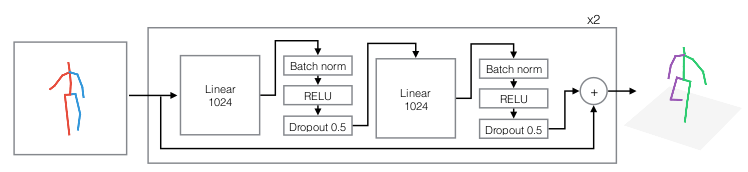
\includegraphics[width = 0.95\textwidth]{linear_figure}
	\caption{Linear model from~\parencite{martinez2017simple}}
	\label{fig_linear_model}
\end{figure}

Loss-function, basicly MSE:
\begin{equation}
	MSE(\widehat{Y}, Y) = \frac{1}{N}\sum_{n = 1}^N \rVert \widehat{Y}_{n} - Y_{n} \lVert_2^2
\end{equation}

\subsection{Sequence-to-sequence model}

\begin{figure}[H]
	\centering
	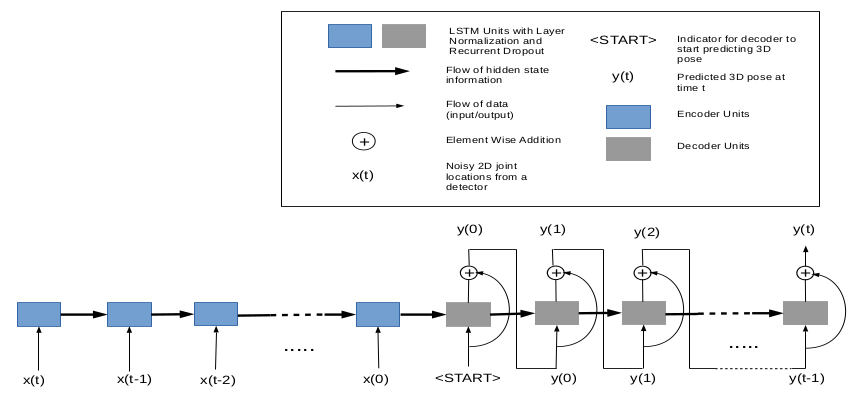
\includegraphics[width = 0.95\textwidth]{seq2seq_figure}
	\caption{Sequence-to-sequence model from~\parencite{hossain2017exploiting}}
	\label{fig_seq2seq_model}
\end{figure}

Loss-function, MSE over time + temporal constraint:
\begin{equation}
	\bm{\mathcal{L}} = \frac{1}{N}\sum_{n=1}^N\left(\frac{\alpha}{T}\sum_{t=1}^T\rVert \widehat{Y}_{n,t} - Y_{n,t} \lVert_2^2 + \frac{\beta}{T-1}\sum_{t = 1}^{T-1}\lVert \widehat{Y}_{n,t + 1} - \widehat{Y}_{n,t}\rVert_2^2\right)
\end{equation}

\begin{enumerate}
	\item Attention mechanism in seq2seq ?
	\item 
\end{enumerate}

\subsection{Results}

\begin{table}
	\begin{tabular}{*{9}{c}}
		\toprule
		model & direction & discussion & eating & greeting & phoning & photo & posing & purchases\\
		\midrule
		linear         & 51.8 & 56.2 & 58.1 & 59.0 & 69.5 & 78.4 & 55.2 & 58.1 \\
		seq2seq         & 44.2 & 46.7 & 52.3 & 49.3 & 59.9 & 59.4 & 47.5 & 46.2 \\
		\bottomrule
	\end{tabular}

	\vspace{1cm}

	\begin{tabular}{*{9}c}
		\toprule
		 model & sitting & sittingdown & smoking & waiting & walkdog & walking & walktogether & Avg\\
		 \midrule
		 linear & 74.0 & 94.6 & 62.3 & 59.1 & 65.1 & 49.5 & 52.4 & 62.9  \\
		 \midrule
		 seq2seq  & 59.9 & 65.5 & 55.8 & 50.4 & 52.3 & 43.5 & 45.1 & 51.9 \\
	\end{tabular}
	\caption{Erros action-wise on Human3.6M dataset from 2D pose estimates from stacked-hourglass network~\parencite{newell2016} as reported in~\parencite{hossain2017exploiting}}
	\label{tab_res_sh_to_3d}
\end{table}


\begin{table}
	\begin{tabular}{*{9}{c}}
		\toprule
		model & direction & discussion & eating & greeting & phoning & photo & posing & purchases\\
		\midrule
		linear & 37.7 & 44.4 & 40.3 & 42.1 & 48.2 & 54.9 & 44.4 & 42.1  \\
		seq2seq  & 35.2 & 40.8 & 37.2 & 37.4 & 43.2 & 44.0 & 38.9 & 35.6 \\
		\bottomrule
	\end{tabular}

	\vspace{1cm}

	\begin{tabular}{*{9}c}
		\toprule
		 model & sitting & sittingdown & smoking & waiting & walkdog & walking & walktogether & Avg\\
		 \midrule
		 linear  & 54.6 & 58.0 & 45.1 & 46.4 & 47.6 & 36.4 & 40.4 & 45.5 \\
		 seq2seq & 42.3 & 44.6 & 39.7 & 39.7 & 40.2 & 32.8 & 35.5 & 39.2 \\
	\end{tabular}
	\caption{Erros action-wise on Human3.6M dataset from 2D ground-truth poses as reported in~\parencite{hossain2017exploiting}}
	\label{tab_res_sh_to_3d}
\end{table}

\printbibliography

\end{document}
